\documentclass{article}

\usepackage{Sweave}
\begin{document}
\Sconcordance{concordance:04_analysis.tex:04_analysis.Rnw:%
1 2 1 1 0 20 1}




\section{Analysis}

\subsection{Exploratory Data Analysis}
Before building our model, we first wanted to understand the data that we were building our model on. Below, I've hsown the summary statistics for the quantitative variables as well as histograms for ACT scores, SAT scores, and graduation rates. 

\input{quantitative_summary, file = '../../data/eda.txt'}
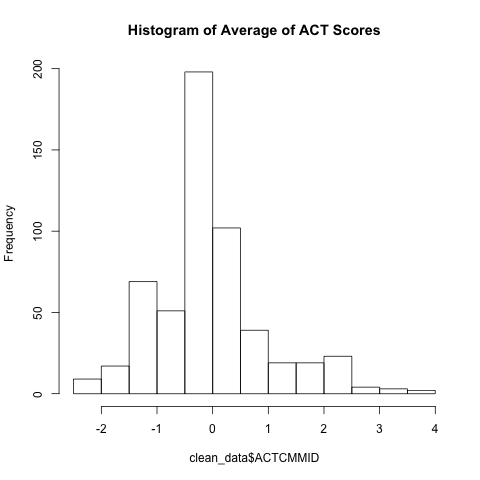
\includegraphics{../../images/histogram_ACT_avg.png}
The maximum score for the ACT is 36.
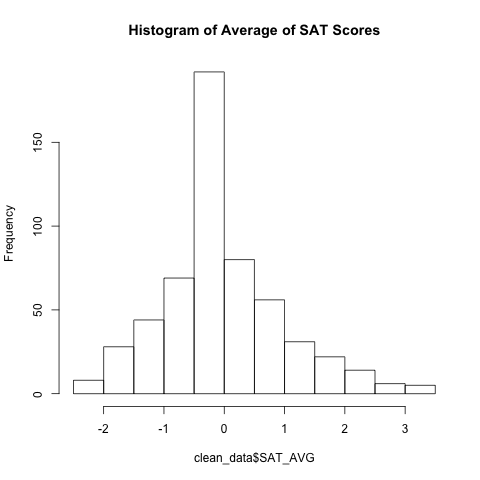
\includegraphics{../../images/histogram_SAT_avg.png}
The maximum score for the SAT is 2400.
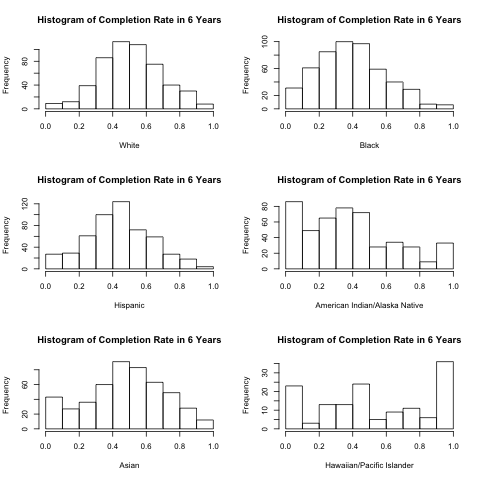
\includegraphics{../../images/histogram_race_completion}
The histogram above depics graduation rates for each ethnicity. 
The total score of the SAT is 2400.
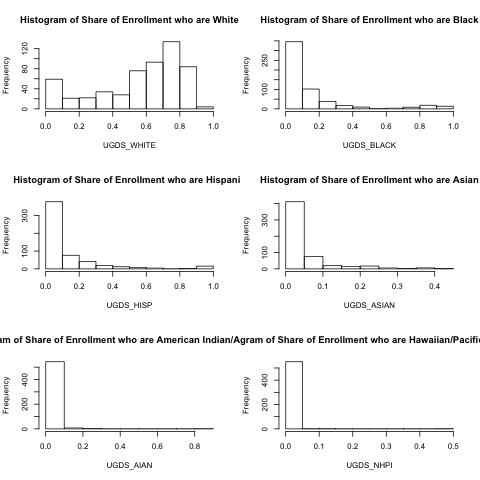
\includegraphics{../../images/histogram_race_enrollment.png}
Comparing the histograms of enrollment by race, it is obvious that the white population has the most enrollment and American Indian/Alaska Native and Hawaiian/Pacific Islander has the least enrollment.
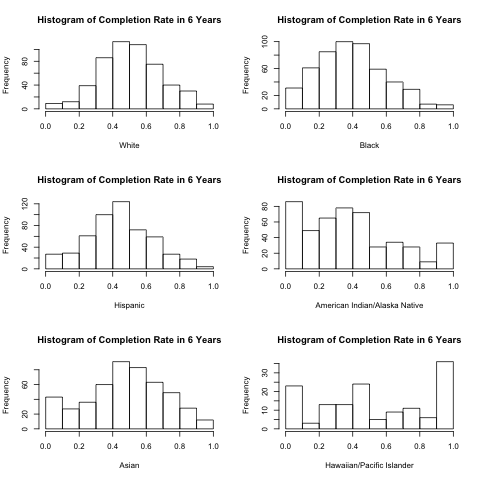
\includegraphics{../../images/histogram_race_completion}
Last but not least, comparing the histograms of completion rate by race, the White, Black, Hispanic, and Asian populations shows a more normal distibution while the American Indian/Alaska Native and Hawaiian/Pacific Islander population are more skewed.

From the above histograms, we can have a general idea of the distribution and maybe which variables affects graduation rate. However, to have a more concrete idea, we want to do further analysis.


\subsection{Variable Selection Methods}

\end{document}
